% Created by tikzDevice version 0.10.1 on 2018-01-12 15:55:47
% !TEX encoding = UTF-8 Unicode
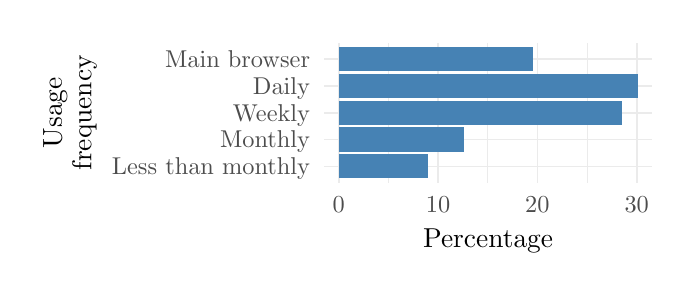
\begin{tikzpicture}[x=1pt,y=1pt]
\definecolor{fillColor}{RGB}{255,255,255}
\path[use as bounding box,fill=fillColor,fill opacity=0.00] (0,0) rectangle (231.26, 86.72);
\begin{scope}
\path[clip] (106.99, 30.77) rectangle (225.76, 81.22);
\definecolor{drawColor}{gray}{0.92}

\path[draw=drawColor,line width= 0.3pt,line join=round] (130.33, 30.77) --
	(130.33, 81.22);

\path[draw=drawColor,line width= 0.3pt,line join=round] (166.23, 30.77) --
	(166.23, 81.22);

\path[draw=drawColor,line width= 0.3pt,line join=round] (202.13, 30.77) --
	(202.13, 81.22);

\path[draw=drawColor,line width= 0.6pt,line join=round] (106.99, 36.59) --
	(225.76, 36.59);

\path[draw=drawColor,line width= 0.6pt,line join=round] (106.99, 46.30) --
	(225.76, 46.30);

\path[draw=drawColor,line width= 0.6pt,line join=round] (106.99, 56.00) --
	(225.76, 56.00);

\path[draw=drawColor,line width= 0.6pt,line join=round] (106.99, 65.70) --
	(225.76, 65.70);

\path[draw=drawColor,line width= 0.6pt,line join=round] (106.99, 75.40) --
	(225.76, 75.40);

\path[draw=drawColor,line width= 0.6pt,line join=round] (112.38, 30.77) --
	(112.38, 81.22);

\path[draw=drawColor,line width= 0.6pt,line join=round] (148.28, 30.77) --
	(148.28, 81.22);

\path[draw=drawColor,line width= 0.6pt,line join=round] (184.18, 30.77) --
	(184.18, 81.22);

\path[draw=drawColor,line width= 0.6pt,line join=round] (220.08, 30.77) --
	(220.08, 81.22);
\definecolor{fillColor}{RGB}{70,130,180}

\path[fill=fillColor] (112.38, 32.23) rectangle (144.69, 40.96);

\path[fill=fillColor] (112.38, 41.93) rectangle (157.76, 50.66);

\path[fill=fillColor] (112.38, 51.63) rectangle (214.84, 60.36);

\path[fill=fillColor] (112.38, 61.33) rectangle (220.36, 70.07);

\path[fill=fillColor] (112.38, 71.04) rectangle (182.53, 79.77);
\end{scope}
\begin{scope}
\path[clip] (  0.00,  0.00) rectangle (231.26, 86.72);
\definecolor{drawColor}{gray}{0.30}

\node[text=drawColor,anchor=base east,inner sep=0pt, outer sep=0pt, scale=  0.88] at (102.04, 33.56) {Less than monthly};

\node[text=drawColor,anchor=base east,inner sep=0pt, outer sep=0pt, scale=  0.88] at (102.04, 43.27) {Monthly};

\node[text=drawColor,anchor=base east,inner sep=0pt, outer sep=0pt, scale=  0.88] at (102.04, 52.97) {Weekly};

\node[text=drawColor,anchor=base east,inner sep=0pt, outer sep=0pt, scale=  0.88] at (102.04, 62.67) {Daily};

\node[text=drawColor,anchor=base east,inner sep=0pt, outer sep=0pt, scale=  0.88] at (102.04, 72.37) {Main browser};
\end{scope}
\begin{scope}
\path[clip] (  0.00,  0.00) rectangle (231.26, 86.72);
\definecolor{drawColor}{gray}{0.30}

\node[text=drawColor,anchor=base,inner sep=0pt, outer sep=0pt, scale=  0.88] at (112.38, 19.76) {0};

\node[text=drawColor,anchor=base,inner sep=0pt, outer sep=0pt, scale=  0.88] at (148.28, 19.76) {10};

\node[text=drawColor,anchor=base,inner sep=0pt, outer sep=0pt, scale=  0.88] at (184.18, 19.76) {20};

\node[text=drawColor,anchor=base,inner sep=0pt, outer sep=0pt, scale=  0.88] at (220.08, 19.76) {30};
\end{scope}
\begin{scope}
\path[clip] (  0.00,  0.00) rectangle (231.26, 86.72);
\definecolor{drawColor}{RGB}{0,0,0}

\node[text=drawColor,anchor=base,inner sep=0pt, outer sep=0pt, scale=  0.99] at (166.37,  7.44) {Percentage};
\end{scope}
\begin{scope}
\path[clip] (  0.00,  0.00) rectangle (231.26, 86.72);
\definecolor{drawColor}{RGB}{0,0,0}

\node[text=drawColor,rotate= 90.00,anchor=base,inner sep=0pt, outer sep=0pt, scale=  0.99] at ( 12.32, 56.00) {Usage};

\node[text=drawColor,rotate= 90.00,anchor=base,inner sep=0pt, outer sep=0pt, scale=  0.99] at ( 23.01, 56.00) {frequency};
\end{scope}
\end{tikzpicture}
